
\documentclass[a4paper,11pt]{article}
\usepackage{float}
\usepackage{listings}
\usepackage{graphicx}
\usepackage{hyperref }
\usepackage[acronym]{glossaries}
%\usepackage[xindy,toc]{glossaries}
\makeglossaries

\title{PyGMO Visualization Manual}
\author{
      Edgar Sim\'{o} Serra \\
      Mentored by Chit-Hong Yam and Dario Izzo 
}
\date{\today}

\newcommand{\HRule}{\rule{\linewidth}{0.5mm}}

\begin{document}
\begin{titlepage}

\begin{center}

\vfill

\vspace*{2 cm}

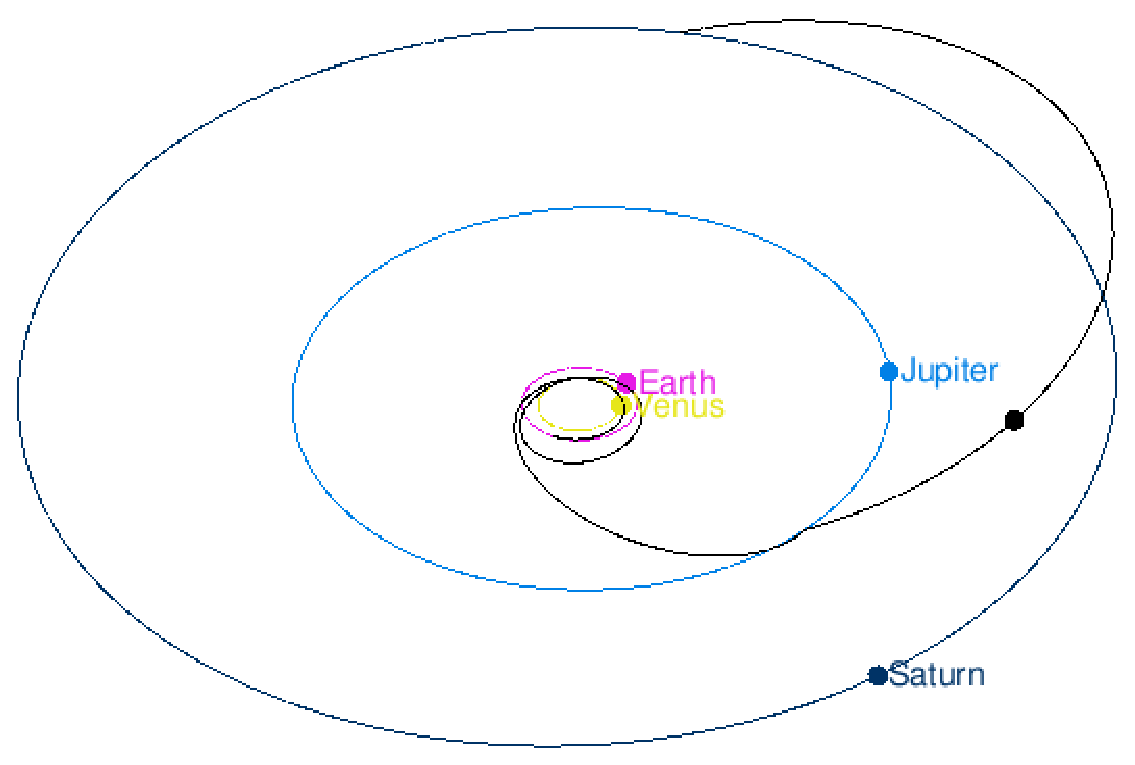
\includegraphics[width=0.25\textwidth]{img/cover}\\[1cm]

\textsc{\LARGE PaGMO}\\[0.5cm]
\HRule \\[0.5cm]
\textsc{\Large PyGMO Visualization Module Manual}\\[0.5cm]
\HRule \\[1.5cm]

% Title
%{ \huge \bfseries Lager brewing techniques}\\[0.4cm]

% Author and supervisor
\begin{minipage}{0.4\textwidth}
\begin{flushleft} \large
\emph{Author:}\\
Edgar Sim\'{o}
\end{flushleft}
\end{minipage}
\begin{minipage}{0.4\textwidth}
\begin{flushright} \large
\emph{Mentors:} \\
Chit Hong Yam \\
Dario Izzo
\end{flushright}
\end{minipage}

\vspace{2 cm}

\includegraphics[width=0.25\textwidth]{img/gsoc2010}\\[1cm]

\vfill

% Bottom of the page
{\large \today}

\end{center}

\end{titlepage}

%\maketitle

\begin{abstract}
Manual for the Visualization module from PyGMO developed for PaGMO as part of the Google Summer of Code 2010 project.
\end{abstract}



\newacronym{API}{API}{Application Programmable Interface}
\newacronym{PaGMO}{PaGMO}{Parallel Global Multiobjective Optimizer}
\newglossaryentry{PyGMO}
{
   name={PyGMO},
   description={Python bindings for PaGMO}
}
\newacronym{GSoC}{GSoC}{Google Summer of Code}
\newglossaryentry{python}
{
   name={Python},
   description={Interpreted, object-oriented, high-level programming language with dynamic semantics}
}
\newglossaryentry{opengl}
{
   name={OpenGL},
   description={Standard specification defining a cross-language, cross-platform API for writing applications that produce 2D and 3D computer graphics}
}
\newacronym{csv}{CSV}{Comma Separated Value}
\newacronym{MGA}{MGA}{Multiple Gravity Assist}
\newacronym{DSM}{DSM}{Deep Space Maneuver}
\newacronym{SI}{SI}{International System of Units}
\newacronym{mjd2000}{MJD2000}{Modified Julian Date 2000}


% The glossary
\printglossaries


\tableofcontents
\newpage


\section{Introduction}
This is the manual for the Visualization module which is part of the \gls{PyGMO} python suite for interaction with \gls{PaGMO}\cite{pagmo}. The objective of this module is 3D Visualization of Interplanetary Trajectories. This manual is intended both for python developers using the PyGMO \gls{API} and end users executing the python script.


\subsection{Requirements}

The main requirement for the visualization module is \gls{python} and \gls{opengl}. Besides this the requirements are very loose. The following should give an approximate idea of what kind of computer is needed to run the visualization module:

\begin{itemize}
\item Pentium II class processor or better
\item 10 MB free dis space
\item 50 MB free RAM
\item OpenGL 1.1 capable card with VBO extension
\end{itemize}

To be able to run the visualization module you must have all the dependencies. The dependency list is:\label{lbl:deps}

\begin{itemize}
\item \gls{python}
\item PyOpengl module
\item numpy module
\item PyFTGL module
\item RE module
\item CSV module
\item dateutil module
\end{itemize}


\subsection{Features}

The Visualization module is designed around flexibility and simplicity. 

\paragraph{Feature list:}
\begin{itemize}
\item Visualization of trajectories
\item Ability to add planets
\item Time slider to be able to move to any time instant in the path
\item Keyboard interaction
\item Mouse Interaction that behaves like most 3D applications
\item Support for processing \gls{csv} files.
\end{itemize}


\section{Installing the Visualization Module}\label{sec:install}

The installation is not different from the standard \gls{PaGMO} and \gls{PyGMO} installation\cite{install:pagmo}. However care must be taken so that \gls{PyGMO} is also installed.


\section{Using the Visualization Module}

The visualization module has two important aspects. The first is the acquiring of the data and setting up of the window. The second is the moving and manipulating of the trajectory with the window.


\subsection{Python API}

The \gls{python} \gls{API} is aimed at developers although it is simple enough to be used by anyone.

\subsubsection{Getting Started}\label{sec:started}

To get started with the python you just have to include the module. If PyGMO is properly installed and your python paths are set correctly you should be able to run the following line in python console or a python script:
\begin{lstlisting}[language=Python,breakatwhitespace=true]
from PyGMO import visualization
\end{lstlisting}
This line will import the visualization module to allow you to get started with it. If no error is thrown that means you have PyGMO properly installed. If you get an error check the troubleshooting guide in section \ref{sec:troubleshoot}.

The next important step to be able to visualize a trajectory is to generate a proper dataset. Datasets are composed of control pointse. Each control point has the following format:

$ t, r, v, dv $

Where $r$, $v$ and $dv$ are vectors of length 3 containing the x, y and z components. They stand for:

\begin{itemize}
\item $t$: Time stamp of the control point. Should be in \gls{mjd2000}\cite{mjd2000} format although the units do not matter as they can be converted.
\item $r$: The position from the common reference which is usually the sun. Has 3 components for the x, y and z vectors.
\item $v$: The velocity with 3 components.
\item $dv$: The delta velocity with 3 components.
\end{itemize}

That means the length of each control point is of 10 values. So each dataset should have a length that is a multiple of 10. Data can be passed either by a tuple or it can be read from a file. The loading data from a file is handled in the advanced \gls{python} in section \ref{sec:advanced}. The simple example dataset taken from example1.py in appendix \ref{app:example1} is the following (numbers truncated so the table fits):

\begin{tabular}{|c|c|c|c|c|c|c|c|c|c|}
   t & r.x & r.y & r.z & v.x & v.y & v.z & dv.x & dv.y & dv.z \\
   8273.2 & 13.52e6 & -67.43e6 & 0. & 13.31 & 30.26 & -1.21 & 0. & 0. & 0. \\
   8623.2 & -242.53e6 & -36.77e6 & 5.20e6 & 5.46 & -19.75 & 0.56 & 0. & 0. & 0. \\
\end{tabular}

Of course these values would have to be formatted as a python list or tuple. We can create the dataset tuple with the following code:

\begin{lstlisting}[language=Python,breakatwhitespace=true]
data = ( 8273.267,
            135299631.153314,
               -67433330.1118738,
               0.,
            13.3117666043686,
               30.2608967735421,
               -1.21905509181638,
            0.,
               0.,
               0.,
         8623.267,
            -242539545.423682,
               -36777066.1865885,
               5209166.99174208,
            5.46701901228146,
               -19.7530014959265,
               0.562626144359047,
            0.,
               0.,
               0. )
\end{lstlisting}

Now that we have the data we have to prepare the conversion ratios so that they get converted to \gls{SI}\cite{siunits} base units. In our case this means seconds for $t$, meters for $r$, meters per second for $v$ and meters per second for $dv$. In this case our dataset we have to convert from days, kilometers, kilometers per second and kilometers per second respectively. So now we proceed to generate the trajectory class with our data:

\begin{lstlisting}[language=Python,breakatwhitespace=true]
traj = visualization.Trajectory3D( data, # Our dataset
      640, 480, # Our window size
      24.*3600., # Conversion from days to seconds
      1000., # Conversion from kilometers to meters
      1000., # Conversion from kilometers per second
             # to meters per second
      1. ) # Conversion from kilometers per second
           # to meters per second
\end{lstlisting}

Now we have created the class object. We can now proceed to manipulate it. For example, if we want to add the planets of earth and mars it's as easy as running the following command:

\begin{lstlisting}[language=Python,breakatwhitespace=true]
traj.addPlanets( [ 'earth', 'mars' ] )
\end{lstlisting}

They will be created using the \gls{mjd2000} dates from the $t$ value of the control points. It is very important that the $t$ value matches the right time otherwise the planets will not by synchronized with the trajectory. To display units again in the original dataset units we can run the $setUnits$ function.

\begin{lstlisting}[language=Python,breakatwhitespace=true]
traj.setUnits( "km", "d", "km/s" )
\end{lstlisting}

This will make the class convert the units when displaying them to the units we just defined. Finally we can mess a bit with the visual aspect of the window before displaying it.

\begin{lstlisting}[language=Python,breakatwhitespace=true]
traj.origin( True ) # Displays the origin axes,
                    # useful for debugging and
                    # getting a reference idea
traj.vectors( True ) # Shows vectors from the moving
                      #object to the origin,
                      useful for debugging
traj.repeat( True ) # Makes the animation repeat itself
traj.axes( True ) # Sets axes that display the values
                  # on the projection of the screen
\end{lstlisting}

When we are satisfied with the tuning of the class we can create the window with the $start$ function.

\begin{lstlisting}[language=Python,breakatwhitespace=true]
traj.start()
\end{lstlisting}

Now the window will be created and show the data. The output of this example can be seen at \ref{img:example1}. The full source code is available at appendix \ref{app:example1}. For more details on how to manipulate the trajectory in the window go to section \ref{sec:window}.


\subsubsection{Advanced}\label{sec:advanced}

While the visualization module may seem simple it has many features that make it much more complex than it seems. One of the most important features is the ability to read from \gls{csv} files. Basically it allows you to import control points and planet flybys from \gls{csv} files.

To load control points from a \gls{csv} file you basically need to define a \gls{csv} file in the same format as the data shown in section \ref{sec:started}. That is to use the following format:

$ t, r, v, dv $

With $r$, $v$ and $dv$ being 3 component vectors. When you have a file in this format you then pass the file name as the data paramaeter when creating a new class. For example example2.py in appendix \ref{app:example2} uses the following:

\begin{lstlisting}[language=Python]
traj = visualization.Trajectory3D( "CassiniMGA.txt", 640, 480,
      24.*3600., 1000., 1000., 1000. )
\end{lstlisting}

It is loading the data from $CassiniMGI.txt$ which is the \gls{csv} file containing the data. Planets can also be loaded this way, however planets are much more powerful this way as you can specify flyby distances and delta velocity of the flyby. The format for the planet \gls{csv} file is the following:

$ name, date, dv, r $

$name$ is the name of the planet which can be one of:

\begin{itemize}
\item Mercury
\item Venus
\item Earth
\item Mars
\item Jupiter
\item Saturn
\item Uranus
\item Neptune
\end{itemize}

$date$ is the date of the flyby. This date can be in any format and the parser will interprete it. If it is just a number it is assumed to be in \gls{mjd2000} as days. $dv$ is the delta velocity of the flyby in kilometers per second and $r$ is the distance of the flyby in kilometers. If $r$ is 'NaN' it assumes that the planet is either the take off or the land planet. An example planet \gls{csv} file would be:

\begin{lstlisting}
Earth,8.3230060190000000E+03,0.,NaN
Earth,9.3718274560000100E+03,0.,7000.0
Jupiter,1.1235668426000000E+04,0.,NaN
\end{lstlisting}

This is example is taken from appendix \ref{app:example2}. The first line is the take off from Earth. The second line is a flyby of earth at 7000 kilometers distance. The third line is the arrival at Jupiter. To load planets from the \gls{csv} file it just has to be passed as the parameter of $addPlanets$ like so:

\begin{lstlisting}[language=Python]
traj.addPlanets( "CassiniMGA_flybyinfo.txt" )
\end{lstlisting}

There is more \gls{API} also available. To read the documentation you can access it with:

\begin{lstlisting}[language=Python]
from PyGMO import visualization
help(visualization)
\end{lstlisting}


%\subsubsection{Common Issues}


\subsection{3D Trajectory Window}\label{sec:window}

The 3D Trajectory Window is composed of many elements. Some of these can be seen in \ref{img:guide}.

\begin{figure}[h]
\centering
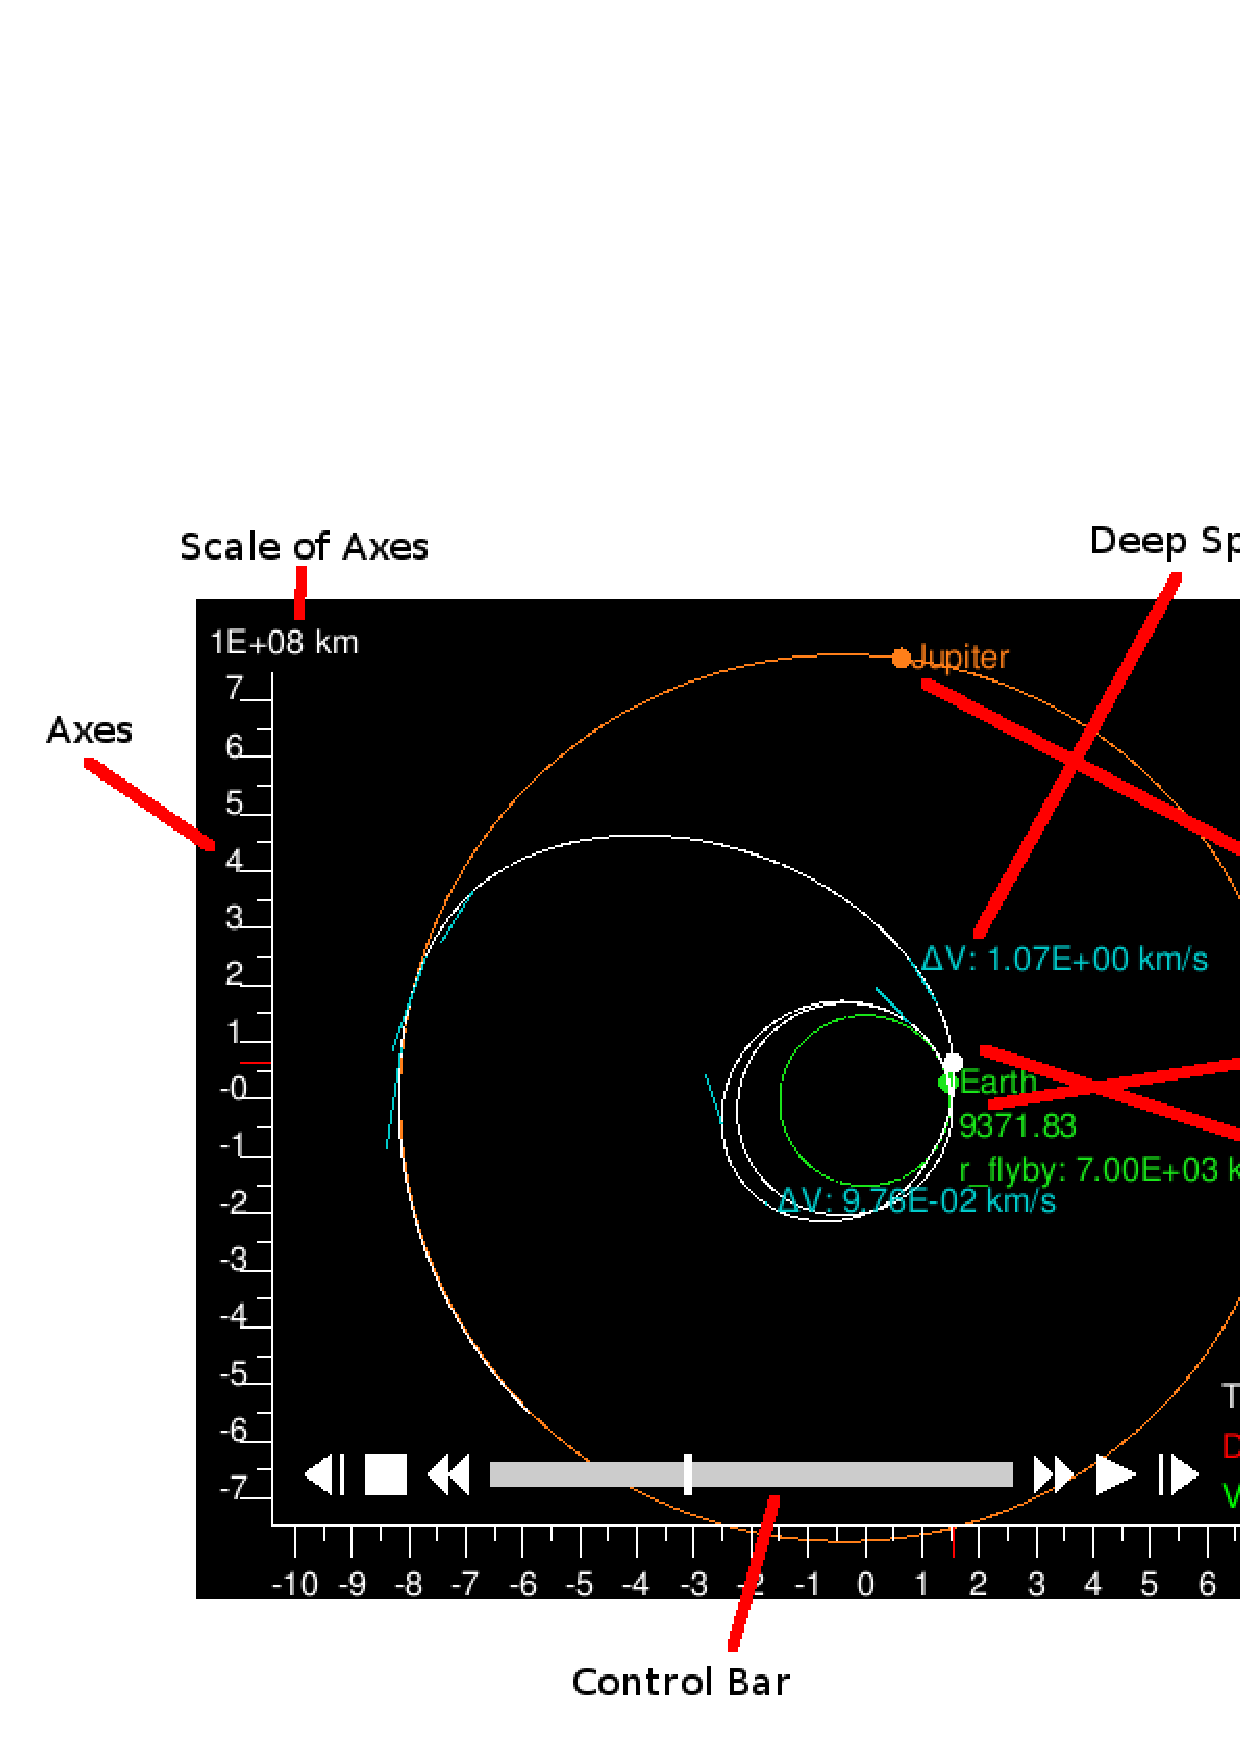
\includegraphics[width=1\textwidth]{img/guide}
\caption{Example of the window elements}
\label{img:guide}
\end{figure}

Many of these elements are optional and can be toggled through the python API when creating the window.

\subsubsection{Mouse}

The mouse is mainly used for moving the camera. The bindings are an unofficial 3D standard:

\begin{itemize}
\item \textbf{Middle Mouse Drag:} Rotates the camera around.
\item \textbf{Control + Middle Mouse Drag:} Moves the camera around.
\item \textbf{Left Mouse Click:} Interacts with the control
\end{itemize}

\subsubsection{Keybindings}

The keybindings are designed for interaction with all sorts of elements. These bindings are grouped into two major grous: camera and playback bindings.

The camera bindings:

\begin{itemize}
\item \textbf{Escape:} Exits.
\item \textbf{q:} Exits.
\item \textbf{Arrow Keys:} Rotates the camera around.
\item \textbf{c:} Resets the camera to isometric and optimizing screen space.
\item \textbf{z:} Zooms in.
\item \textbf{Z:} Zooms out.
\item \textbf{2:} Faces from the bottom (0, 0, -1).
\item \textbf{4:} Faces from the left (0, -1, 0).
\item \textbf{5:} Faces forwards (0, 1, 0).
\item \textbf{6:} Faces from the right (0, 1, 0).
\item \textbf{8:} Faces from the top (0, 0, 1).
\end{itemize}

The playback bindings:

\begin{itemize}
\item \textbf{p:} Toggles pause.
\item \textbf{r:} Restarts playback.
\item \textbf{f:} Accelerates playback.
\item \textbf{s:} Slows down playback.
\item \textbf{h:} Toggles control visibility.
\end{itemize}


%\subsubsection{Common Issues}


\section{Troubleshooting}\label{sec:troubleshoot}

\subsection{Import fails}

If you are getting the following error.

\begin{lstlisting}
>>> from PyGMO import visualization
 Traceback (most recent call last):
   File "<stdin>", line 1, in <module>
   ImportError: No module named PyGMO
\end{lstlisting}

You have not installed PyGMO properly, please refer to section \ref{sec:install} for how to install.


\subsection{Missing dependencies}

If you are getting an error similar to:

\begin{lstlisting}
Warning: The python-opengl bindings are missing, you won't be able to use the visualization module.
\end{lstlisting}

Please double check to make sure you have all the PyGMO dependencies. Refer to section \ref{lbl:deps} for details on the dependencies.


\appendix

\newpage
\section{example1.py}\label{app:example1}
Very simple example of an earth to mars trajectory.
\subsection{Data}
This example does not use external files for data, it declares the data in the code.
\subsection{Code}
\lstinputlisting[language=Python]{../../example1.py}
\subsection{Results}
\begin{figure}[H]
\centering
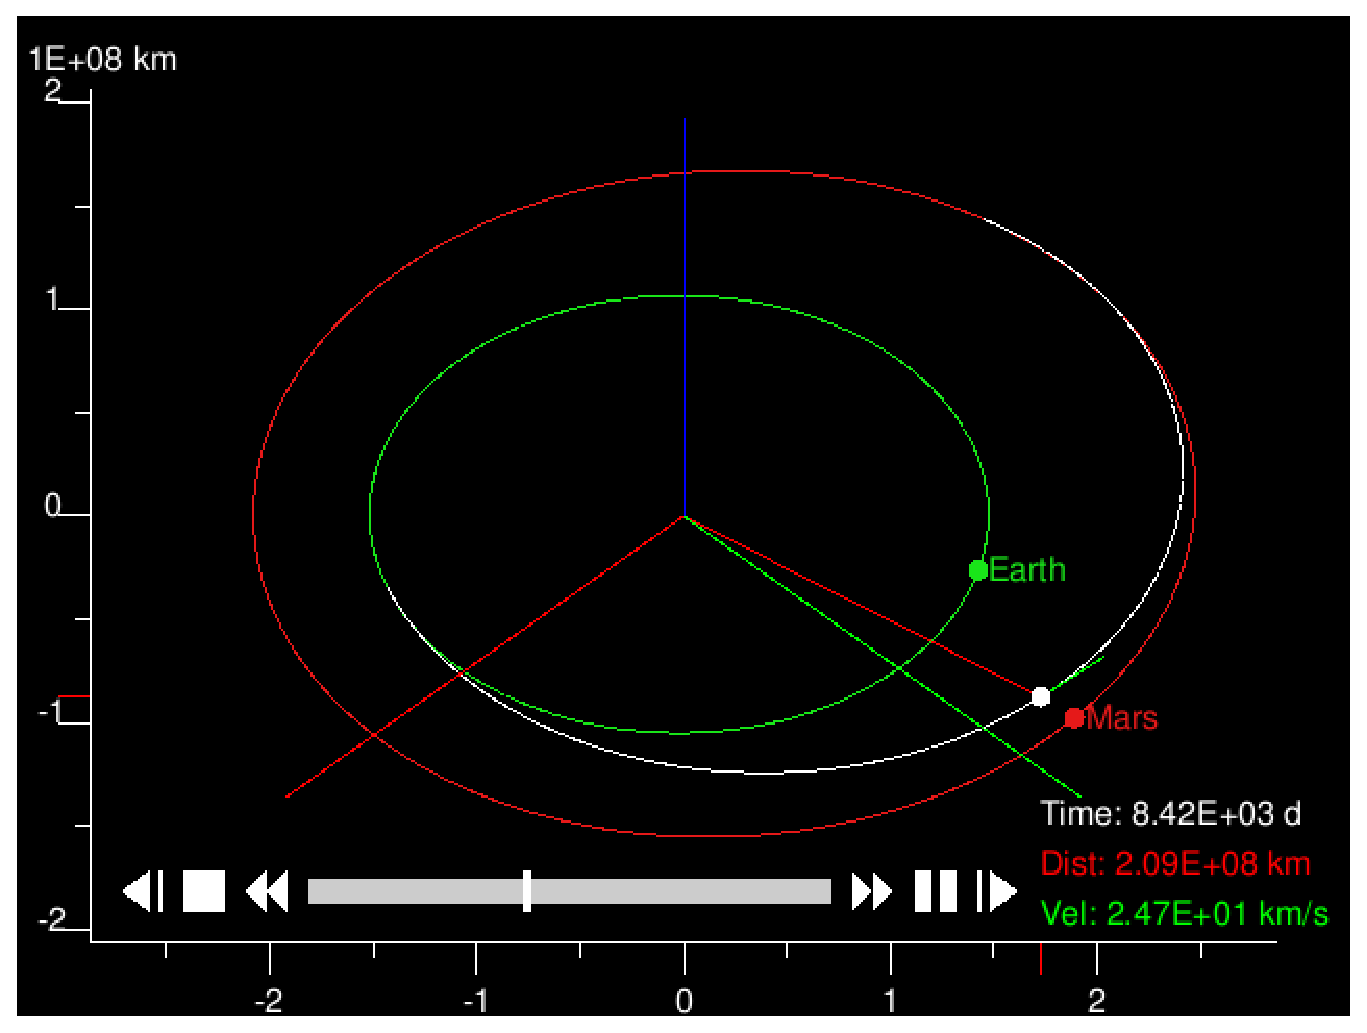
\includegraphics[width=1\textwidth]{img/example1}
\caption{Screenshot of the trajectory from example1.py}
\label{img:example1}
\end{figure}


\newpage
\section{example2.py}\label{app:example2}
Example of doing \gls{MGA}.
\subsection{Data}
For this example we are using:

\begin{itemize}
\item CassiniMGA.txt
\item CassiniMGA\_flybyinfo.txt
\end{itemize}
\subsection{Code}
\lstinputlisting[language=Python]{../../example2.py}
\subsection{Results}
\begin{figure}[H]
\centering
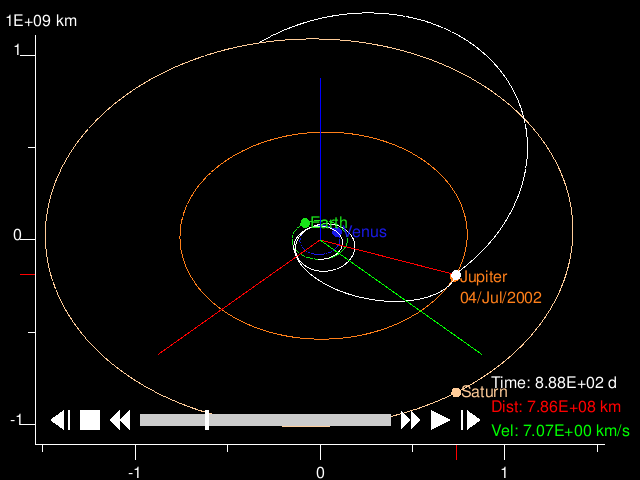
\includegraphics[width=1\textwidth]{img/example2}
\caption{Screenshot of the trajectory from example2.py}
\label{img:example2}
\end{figure}


\newpage
\section{example3.py}
Example of a simple \gls{DSM}.
\subsection{Data}
For this example we are using:

\begin{itemize}
\item EarthMarsDSM.txt
\item EarthMarsDSM\_flybyinfo.txt
\end{itemize}
\subsection{Code}
\lstinputlisting[language=Python]{../../example3.py}
\subsection{Results}
\begin{figure}[H]
\centering
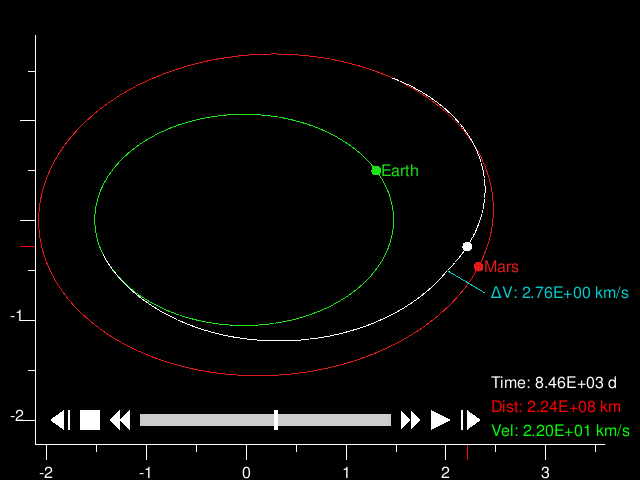
\includegraphics[width=1\textwidth]{img/example3}
\caption{Screenshot of the trajectory from example3.py}
\label{img:example3}
\end{figure}


\newpage
\section{example4.py}
Complete complex dataset example. This one does a gravity assist and multiple \gls{DSM}.
\subsection{Data}
For this example we are using:

\begin{itemize}
\item EarthEarthJupiter.csv
\item EarthEarthJupiter\_flybyinfo.txt
\end{itemize}
\subsection{Code}
\lstinputlisting[language=Python]{../../example4.py}
\subsection{Results}
\begin{figure}[H]
\centering
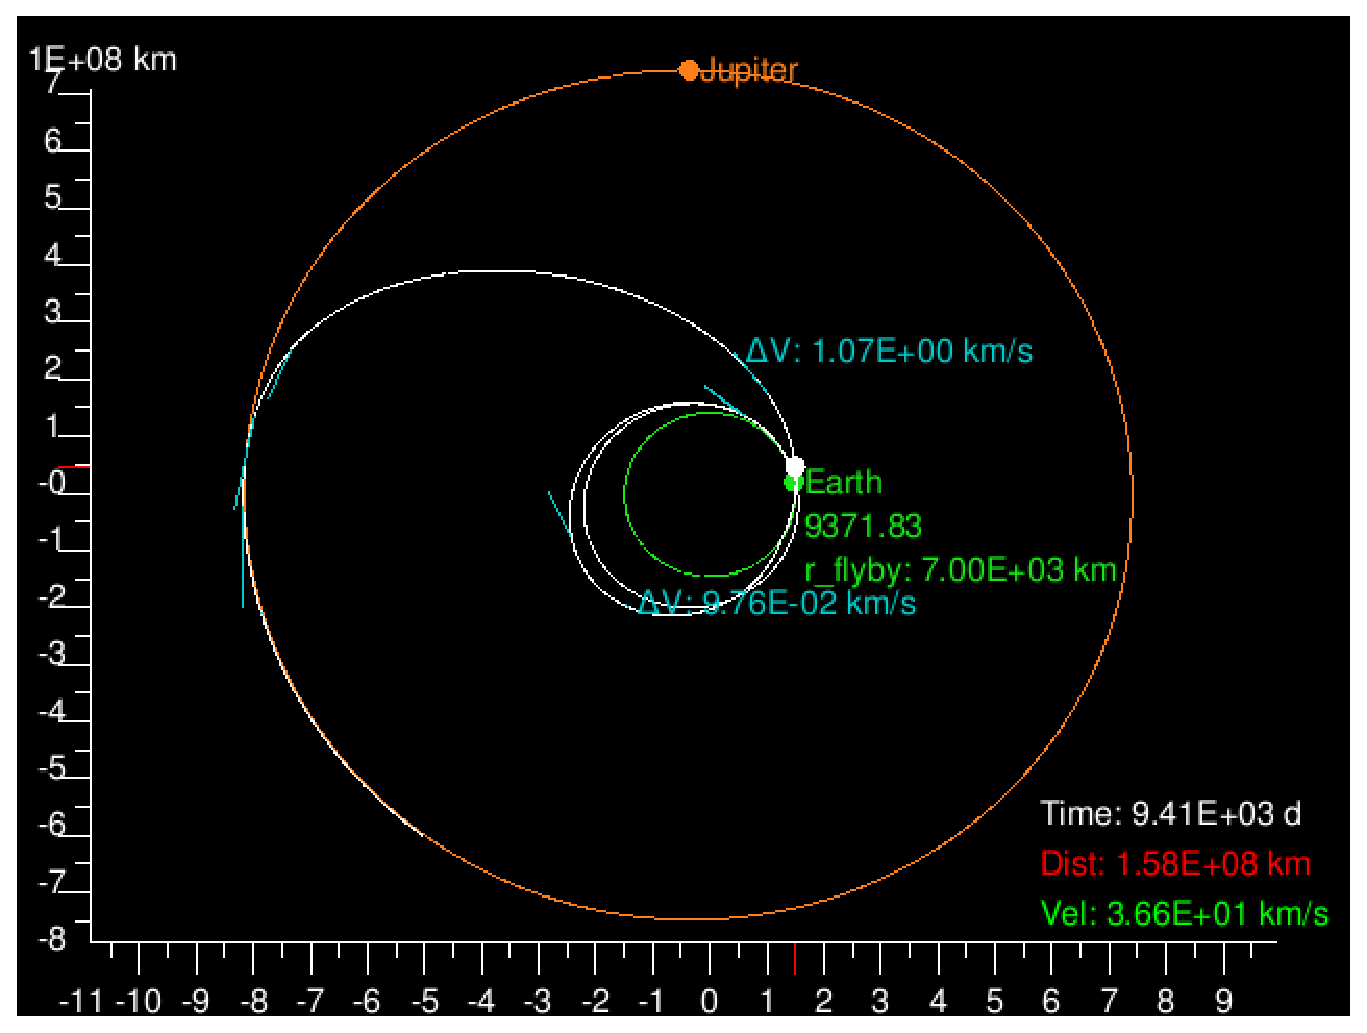
\includegraphics[width=1\textwidth]{img/example4}
\caption{Screenshot of the trajectory from example4.py}
\label{img:example4}
\end{figure}


\bibliographystyle{plain}
\bibliography{manbib}

\end{document}

